\documentclass[11pt,a4paper]{article}
\usepackage[utf8]{inputenc}
\usepackage[T1]{fontenc}
\usepackage[english]{babel}
\usepackage{lmodern,microtype,amsmath,amssymb,booktabs,array,graphicx,xcolor,geometry,setspace,float,longtable}
\usepackage{tikz}
\usepackage[section]{placeins}
\usetikzlibrary{arrows.meta,positioning}
\usepackage[font=small,labelfont=bf]{caption}
\usepackage[authoryear,round]{natbib}
\usepackage[hidelinks]{hyperref}
\geometry{margin=25mm}
\setstretch{1.12}
\setlength{\parskip}{0.35em}
\setlength{\parindent}{1.2em}
\setlength{\emergencystretch}{2em}
\makeatletter
\setlength{\@fptop}{0pt}
\setlength{\@fpsep}{18pt}
\setlength{\@fpbot}{0pt plus 1fil}
\makeatother
\definecolor{reused}{HTML}{1755A0}
\definecolor{revised}{HTML}{B85A00}
\definecolor{added}{HTML}{B02228}
\newcommand{\old}[1]{{\color{reused}#1}}
\newcommand{\rev}[1]{{\color{revised}#1}}
\newcommand{\new}[1]{{\color{added}#1}}
\newenvironment{addition}{\begingroup\color{added}}{\endgroup}
\newcommand{\pp}{percentage points}
\newcommand{\figroot}{../../3. Output/paper_A_2026-09-27/figures/}
\newcommand{\draftlegend}{\begin{center}\small\color{black}Coauthor working draft --- 27 September 2026\\Reference: reviewed 21-page manuscript, before this round of changes.\\\old{Blue: wording retained verbatim.}\quad\rev{Orange: revised existing material.}\\\new{Red: new text or analysis.} Figure frames and captions indicate provenance; plotted colors do not.\end{center}}
\newcommand{\authors}{\old{Ignacio Garijo-Campos} \and \old{Antonio Alfonso} \and \old{Pablo Bra\~nas-Garza} \and \old{Diego Jorrat} \and \old{Angel Sanchez}}
\newcommand{\plot}[4]{\begin{figure}[!htbp]\centering\begingroup\color{#1}\setlength{\fboxsep}{2pt}\fbox{\includegraphics[width=.94\linewidth]{\figroot#2.png}}\caption{\textcolor{#1}{#3}}\label{#4}\endgroup\end{figure}}
\newcommand{\tabnote}[1]{\par\smallskip{\footnotesize\noindent\textit{Notes:} #1\par}}
\newcommand{\inputtab}[4]{\begin{table}[!htbp]\centering\begingroup\color{#1}\caption{\textcolor{#1}{#3}}\label{#4}\small\input{tables/#2.tex}\endgroup\end{table}}
\date{}
\renewcommand{\floatpagefraction}{0.8}
\renewcommand{\topfraction}{0.9}
\renewcommand{\textfraction}{0.07}
\makeatletter\newcommand{\sectionfloatbarrier}{\ifx\@deferlist\@empty\else\clearpage\fi}\makeatother

\title{\rev{Common Criteria, Different Decisions: Student Information and Teacher Harshness in Grade-Repetition Recommendations}}
\author{\authors}
\begin{document}
\maketitle\draftlegend
\color{revised}
\begin{abstract}
Teachers may agree about which student characteristics matter while disagreeing about whether the same student should repeat a grade. We examine this distinction using 22,124 recorded recommendations from 2,705 teachers in Castilla-La Mancha, Spain. Within-teacher comparisons show that failed subjects and low basic competences dominate recommendations, with additional contributions from attendance and discipline. Student gender has a small average coefficient, while a complex social background reduces recommendations of repetition. Disagreement is greatest when several failed subjects coexist with adequate competences: two teachers evaluating the same recorded profile disagree in 49.1 percent of pairs. We summarize teachers' relative recommendations through a card-adjusted measure of harshness. Its correlation across repeated random response halves averages 0.48. Professional characteristics and reported beliefs nevertheless explain little of its variation: full linear and ridge models achieve out-of-sample $R^2$ values of about 3.7 percent. A complementary multilevel decomposition finds residual variation between teachers beyond that associated with their measured characteristics. The findings distinguish the information that changes recommendations, the cases that divide teachers, and the limited ability of observed teacher profiles to anticipate their judgments.
\end{abstract}
\noindent\textbf{Keywords:} grade repetition; teacher judgment; vignette experiment; harshness; disagreement; prediction.

\section{Introduction}
\old{Grade-repetition recommendations translate several kinds of evidence into a binary educational judgment. Failed subjects may indicate that a student has not met the requirements for progression. Basic competences provide a partly different signal of what the student can do. Attendance, classroom behavior, and background can further shape how a teacher interprets the difficulty. Even when teachers broadly agree that academic performance should matter, they may disagree about how much evidence is enough, which evidence should take precedence, and whether repetition is an appropriate response.}

The distinction matters because observed repetition rates combine the situations students face with the judgments applied to those situations. Teachers working with different students can have different repetition rates even if they use the same criteria. Conversely, teachers evaluating comparable students may reach different conclusions. Standardized student profiles allow us to separate these questions more directly than comparisons of classroom repetition rates. A teacher whose actual pupils rarely vary in family circumstances, for example, can evaluate hypothetical pupils from contrasting backgrounds.

The educational case for repetition is itself contingent. Reviews of its consequences document substantial variation across research designs and settings \cite{allen,goos}. Evidence that a student faces academic difficulties therefore does not uniquely determine whether repetition is an appropriate response. Our conceptual framework distinguishes teachers' assessment of difficulties if the student progresses from their assessment of the gains and costs of making the student repeat. This distinction organizes the interpretation of academic signals, behavioral information and social circumstances without assuming that one recommendation is universally correct.

We study 2,705 teachers evaluating profiles with six attributes. The analysis addresses three connected questions. First, which attributes change recommendations within teachers? Second, how much do teachers differ when the information is comparable, and which cases divide them? Third, how much of these differences can be characterized or predicted from teachers' professional characteristics and beliefs? A measure of \textit{harshness}, defined as the average deviation from other teachers' recommendations on the same cards, connects the second and third questions.

\old{Studying these questions together helps distinguish disagreement on individual cases from broader patterns in teachers' recommendations. Disagreement over one student profile need not imply that the same teachers also differ across other profiles. If some teachers repeatedly recommend retention more often than their peers on comparable cases, however, there is a pattern to explain---even if their observed characteristics provide little help in predicting it.}

The results distinguish all three levels. Failed subjects and low competences have the largest within-teacher coefficients, 54.6 and 27.1 percentage points, and reinforce one another in an interaction specification. Attendance and discipline also matter. Gender has a small average coefficient, and complex social background moderates repetition recommendations. These last two findings contrast with the higher repetition incidence among boys and disadvantaged students documented in population data \cite{oecd}. Such disparities need not take the form of an additional penalty when teachers assess otherwise comparable profiles.

Harshness varies substantially across teachers, and their relative position shows moderate consistency across different subsets of their answers. Disagreement is especially pronounced for several failed subjects combined with adequate competences. Yet demographic and professional information, together with reported beliefs, yields only modest prediction of harshness in teachers held out of estimation. A complementary decomposition of decisions distinguishes the large contribution of student information from a remaining teacher component that measured characteristics do not capture. The contribution is thus to connect common criteria, disagreement on comparable cases and the limits of predicting who will be more severe.

\section{Related literature}
The first literature concerns the consequences of retaining students. Allen et al.\ \cite{allen} find less negative estimated achievement effects in stronger research designs. Goos et al.\ \cite{goos} report an average effect near zero alongside heterogeneity across contexts, comparisons and outcomes. These findings motivate attention to how teachers make recommendations; they do not supply a universal decision rule for every student profile. Studies of recommendations and studies of the consequences of actual retention address complementary questions.

Research on teachers' beliefs provides a second foundation. Tomchin and Impara \cite{tomchin} examine the reasoning underlying retention judgments, and Bonvin \cite{bonvin} connects attitudes and judgments to retention decisions. This work motivates our distinction between diagnosing a difficulty and considering repetition an appropriate response. Beliefs are not a single construct: reports of empathy, views about the role of effort and assessments of educational resources capture different considerations \cite{pajares}. We use these measures to characterize observed harshness and assess its predictability.

Klapproth and Beyte \cite{klapproth} provide a close experimental antecedent. Their 146 participants, including 108 teachers in training and 38 practicing teachers, evaluate profiles varying in grades, subject of failure and gender. They also complete a 16-item retention-attitude questionnaire. Both studies use vignettes to connect student information and teacher characteristics to recommendations. Our larger sample of practicing teachers permits a more detailed study of disagreement and prediction. The profile design adds attendance, discipline and social context, and distinguishes failed subjects from basic competences. It therefore addresses conflicts between formal performance and competence rather than differences between subject domains. Our broader professional information and beliefs extending beyond retention also answer a different measurement question; their questionnaire measures retention-specific attitudes more intensively. Weak prediction with our measures would not contradict an association with their more specific attitude instrument.

Multidimensional vignette designs allow researchers to study how several characteristics jointly enter a judgment \cite{conjoint}. Here, variation within teachers identifies changes in recommendations, while repeated profiles locate disagreement across teachers. We complement these comparisons with an explicit assessment of how well teacher information predicts harshness for respondents not used to fit the model. This separates explanatory associations in the observed sample from performance on new observations \cite{prediction}.

\section{Study design and measurement}
\subsection{Participants and questionnaire}
The survey was collected between 14 March and 29 April 2025 among primary and secondary teachers in Castilla-La Mancha. The study plan specifies recruitment through the regional education authority and schools forwarding an online questionnaire. Participation was voluntary. The raw export contains 4,942 records, of which 4,553 remain after the existing screening rule; 2,705 contain at least one usable recommendation. Appendix~\ref{app:sample} combines the participant flow, response availability, timing diagnostics and comparisons with regional teacher statistics.

The questionnaire first collects personal and professional information, then introduces the decision task through examples and eight intended experimental cards, and subsequently elicits beliefs. Each decision is a binary recommendation of promotion or repetition. The six coded attributes are gender, complex social background, failed subjects, basic competences, frequent unjustified absence and serious disciplinary problems. We follow the authors' definition of the background attribute as complex social circumstances, not migrant status.

\begin{figure}[!htbp]\centering\color{revised}
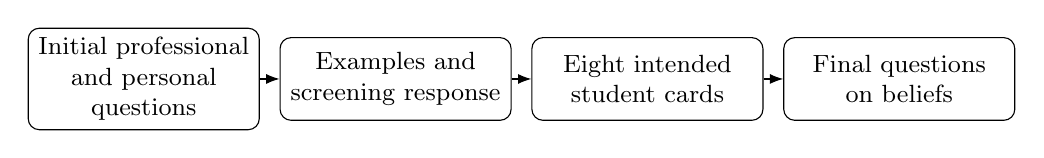
\begin{tikzpicture}[n/.style={draw,rounded corners,align=center,text width=2.7cm,minimum height=1.05cm,font=\small},>=Latex]
\node[n] (a) {Initial professional\\and personal questions};
\node[n,right=0.25cm of a] (b) {Examples and\\screening response};
\node[n,right=0.25cm of b] (c) {Eight intended\\student cards};
\node[n,right=0.25cm of c] (d) {Final questions\\on beliefs};
\draw[->] (a)--(b);\draw[->] (b)--(c);\draw[->] (c)--(d);
\end{tikzpicture}
\caption{\rev{Timing of the measurements used here, within one survey encounter. Belief reports follow the recommendations. Shared-study assignments are described briefly in Appendix~\ref{app:sample}.}}\label{fig:timeline}
\end{figure}
Figure~\ref{fig:timeline} distinguishes initial characteristics from later belief reports. The favorable example serves as a screen: records recommending repetition on its corresponding screening fields are excluded under the existing cleaning rule. Other recorded recommendations, including unfavorable-example information, remain in the analysis. This preserves the response definition used throughout the project. There are 1,736 teachers with nine retained responses, 633 with eight and 336 with one to seven; these are recorded responses, not nine experimental cards. Where a question field was reused, the export does not separately recover its example and experimental answers.

\subsection{Teacher information and analysis samples}
The professional and demographic set, $X_1$, includes educational stage, experience, gender, age, school ownership, a reported permanent public appointment and number of teaching groups. We retain age and experience jointly because they describe different aspects of a career; school tenure is omitted because local institutional integration is not the principal question. The age coefficient compares teachers with equal experience, while the experience coefficient compares teachers of equal age.

$X_2$ adds perceived teacher impact, self-reported empathy and attribution of economic position in Spain to effort rather than luck. The effort scale runs from 1 (luck, family circumstances and contacts) to 10 (effort, education and merit). $X_3$ adds agreement that too many resources are allocated to repeaters, on the original 0--10 scale. This is a single distributive judgment, not a resource-skepticism composite. The item referring to ineffective additional resources is not included.

The existing harmonization combines alternative school/regional versions of the impact and resource questions. Empathy reports on the 0--100 scale are mapped into five categories and combined with the 1--5 version. A permanent public appointment is defined by the response categories actually recorded; its absence does not imply a temporary private-sector contract. The models compare all three predictor sets on the same 2,157 complete cases. A secondary prediction analysis uses the 2,642 teachers with complete $X_1$ information. Missing final beliefs are not replaced with invented responses.

\section{Decision framework and empirical strategy}
\subsection{Diagnosing difficulty and choosing an educational response}
\begin{addition}
A recommendation to repeat can reflect both concern about progression and a view about what repetition would accomplish. Let $x_i$ denote student $i$'s profile. Teacher $j$ perceives a probability $q_j(x_i)$ of consequential difficulty if the student progresses, a gain $g_j(x_i)$ from repetition rather than progression when that difficulty occurs, and a cost $c_j(x_i)$ of repetition. A compact decision rule is
\[
Y_{ij}=\mathbf{1}\{q_j(x_i)g_j(x_i)>c_j(x_i)\}.
\]
This representation concentrates benefits in the event of difficulty and measures benefits and costs on a compatible scale. It is a conceptual simplification, not a claim that teachers consciously calculate these quantities. Their judgments may depend on observed characteristics and beliefs $z_j$, as well as unobserved considerations $\eta_j$. For example, $q_j(x_i)=q(x_i,z_j,\eta_j^q)$; the same dependence applies to gains and costs.

The distinction supplies three useful implications. First, teachers can agree that a student faces difficulties but disagree about whether repeating is the appropriate response. Second, a difficult social context can increase concern about progression while also increasing the perceived costs of retention or reducing its expected gains. A negative background coefficient therefore need not indicate less concern about the student. Third, a common average tendency does not exhaust differences of judgment: teachers with similar harshness can disagree about which students should repeat.

Academic performance informs both the diagnosis and the possible benefit of repeating. Attendance and disciplinary problems can inform assessments of readiness, engagement and how another year would work. Gender and social circumstances can affect interpretations of the same information. We do not assign any attribute or belief item exclusively to one mechanism. The data observe recommendations, not separate measures of $q$, $g$ and $c$. The framework organizes the contrasts and their interpretation rather than claiming to identify these quantities structurally.
\end{addition}

\subsection{Within-teacher responses to student information}
We estimate linear probability models with teacher fixed effects and standard errors clustered by teacher. The fixed effects absorb differences in average recommendation levels; the attribute coefficients summarize changes across the cards a teacher evaluates. Teachers with only one usable response contribute to descriptive harshness but not to identification of these coefficients. The main specification therefore contains 22,006 decisions from 2,587 teachers.

The additive model includes all six attributes. An interaction model adds failed subjects interacted with competences, absence and discipline, with Holm adjustment across those three interaction tests. We retain the recorded profile support rather than filling in unobserved combinations. Appendix~\ref{app:sample} documents the coding and a restricted control-sample check. The within-teacher analysis answers which information changes recommendations; it is distinct from estimating how observed teacher characteristics relate to their average recommendations.

\subsection{Harshness and disagreement between teachers}
We define \textit{harshness} as the teacher's relative propensity to recommend repetition on the cards answered. For each response, the comparison is the repetition rate among other teachers evaluating the same recorded card:
\[
d_{ij}=Y_{ij}-\overline Y_{i,-j},\qquad
H^b_j=\frac{1}{n_j}\sum_{i\in I_j}d_{ij}.
\]
A value of 0.10 means ten percentage points above the references for those cards, on average. The label does not imply that recommending repetition is wrong. Comparing with the same-card reference accounts for the observed profile mix, while the finite number of responses limits how precisely each teacher can be measured.

We present the distribution of $H^b$ before describing its empirical terciles. Ties are retained together, giving groups of 908, 864 and 933 teachers. The tercile regressions describe how attribute coefficients vary across the observed distribution; they do not identify three externally defined types of teacher. A separate check asks whether harshness is consistent across two nonoverlapping subsets of a teacher's responses. We repeat 1,000 random splits among teachers with at least eight responses, using reference samples external to the evaluated teachers and disjoint between the two halves. Appendix~\ref{app:harshness} explains this procedure and its relation to alternative harshness definitions.

Harshness summarizes the direction of a teacher's departures from peers. Same-profile disagreement instead asks whether two distinct teachers evaluating an identical identifier recommend different outcomes. We calculate this probability within each identifier and average it by observed response frequency, including within four categories formed by failed subjects and competences. The two statistics are complementary: similar average harshness need not imply agreement on individual students.

\subsection{Characterization, prediction and sources of variation}
Harshness is the dependent variable in the teacher-level characterization and prediction models. OLS associations use HC3 intervals, supplemented by 999 teacher bootstrap draws that reconstruct card references. Prediction uses five repetitions of five teacher folds. All methods are evaluated on identical targets and partitions within each population. A held-out teacher contributes neither to training nor to the card reference against which that teacher's answers are evaluated.

We compare a training-mean baseline with OLS, ridge regression and random forests \cite{rf}. The last two allow, respectively, regularization and flexible nonlinear relationships. Tuning takes place in three inner teacher folds, with card references reconstructed inside each split. We report prediction error and out-of-sample $R^2$, keeping detailed tuning, paired comparisons and SHAP diagnostics \cite{shap} in Appendix~\ref{app:prediction}. These analyses ask how well the available measures anticipate harshness rather than treating a significant coefficient as evidence of accurate individual prediction.

\begin{addition}
A complementary multilevel model returns to the individual binary decision. It combines student attributes and the failures--competences interaction, professional/demographic characteristics, beliefs, assignment-context indicators and a residual teacher intercept. The intercept represents response-level commonality within teachers that remains after the observed variables. It is related conceptually to unobserved judgment heterogeneity, but is not identical to harshness or to its regression residual.

We partition the model-implied variance into the fitted systematic component, residual teacher variance and remaining decision variance \cite{nakagawa,stoffel}. Within the systematic component, a Shapley allocation averages the incremental contribution of each information block across all orders of entry \cite{groemping}. Our implementation allocates the variance of the full fitted systematic predictor through projections onto subsets of its design columns; it does not sum overlapping partial $R^2$ values. Assignment context remains a separate adjustment block. A linear mixed model provides a response-scale working decomposition with teacher-bootstrap intervals; logistic specifications check the dependence on the binary-response model and scale. Appendix~\ref{app:prediction} gives the exact construction. The decomposition describes fit under a model and is separate from out-of-sample prediction of harshness.
\end{addition}

\section{Results}
\subsection{Within teachers: how student information changes recommendations}
The within-teacher coefficients in Table~\ref{tab:attr} show a clear hierarchy of information. Three or more failed subjects increase the recommendation probability by 54.62 percentage points (95 percent interval 53.23 to 56.01), and low basic competences by 27.07 points (25.83 to 28.31). The control-only estimates have similar magnitudes. These academic indicators convey different information: failed subjects refer to formal performance, whereas competences describe preparedness more broadly.
\inputtab{revised}{attributes}{Within-teacher responses to student attributes}{tab:attr}

Attendance and conduct retain a role beyond the academic indicators. Frequent unjustified absence adds 6.37 points, and serious disciplinary problems add 4.56 points. Their smaller magnitudes do not make them incidental controls: teachers incorporate information about the student's engagement and behavior when deciding between promotion and repetition. The coefficients alone do not distinguish whether this reflects expected educational gains, perceived readiness or normative considerations about conduct.

The male-student coefficient is 0.26 points, with a 95 percent interval from $-0.62$ to 1.15. A complex social background reduces repetition recommendations by 1.88 points (interval $-2.74$ to $-1.02$). The narrow average gender contrast and the negative background coefficient contrast with the higher population incidence of repetition among boys and disadvantaged students \cite{oecd}. Our results are compatible with some observed disparities arising from the academic and school circumstances students bring to the promotion decision, rather than an additional penalty attached directly to their group. The background result is also compatible with a compensatory consideration of difficult circumstances. This does not establish the absence of discrimination throughout schooling or quantify the origins of population gaps.

The interaction specification in Table~\ref{tab:interactions} adds a second feature of the academic pattern. Failed subjects and low competences reinforce one another: their interaction is 10.56 points (8.17 to 12.95). The low-competence contrast is 21.66 points when the failed-subject indicator is absent and 32.22 points when it is present. Interactions of failures with attendance or discipline are smaller and imprecise. This combination of signals is consistent with cumulative academic concern on the probability scale. We next examine whether the shared hierarchy nevertheless leaves teachers divided on particular cases.
\inputtab{revised}{interactions}{Combining academic and behavioral information within teachers}{tab:interactions}

\subsection{Between teachers: harshness, contested cases and descriptive terciles}
Figure~\ref{fig:harshness} introduces the distribution of harshness. Its standard deviation is 20.97 percentage points, and its unweighted mean is $-0.61$ points. The adjustment compares each teacher with peers on the same recorded cards; the unequal numbers of responses explain why the unweighted mean need not be exactly zero. The distribution is not well summarized by the fraction of teachers who recommend repetition in every case or in none: such patterns combine judgment with which cards and how many responses are observed.
\plot{revised}{harshness_distribution}{Distribution of harshness among 2,705 teachers. Higher values indicate more repetition recommendations relative to other teachers evaluating the same cards.}{fig:harshness}

Harshness exhibits moderate consistency within the task. Across 1,000 random splits of each eligible teacher's answers, the correlation between halves averages 0.483. The central 95 percent of partition correlations runs from 0.461 to 0.504. These are different divisions of the same responses, not repeated surveys or a sampling confidence interval. Figure~\ref{fig:halves} in Appendix~\ref{app:harshness} shows the distribution and explains the independent reference construction. The result supports a recurring component in the observed differences without turning a short questionnaire into a precise measure of a permanent trait.

Same-profile disagreement shows where teachers' judgments diverge. Across all recorded identifiers, its frequency-weighted value is 25.89 percent. Table~\ref{tab:academic} locates the principal boundary: for several failed subjects combined with adequate competences, the probability that two teachers disagree on the same identifier is 49.11 percent. When neither academic difficulty is present, disagreement is only 5.81 percent. Recommendation rates also differ asymmetrically across the two conflicting categories: 51.52 percent for several failures with adequate competences, compared with 23.79 percent for low competences with few failures. These contrasts explain why a large average response to academic information need not produce agreement when the signals conflict.
\inputtab{revised}{academic}{Academic profiles and disagreement on the same recorded card}{tab:academic}

Tables~\ref{tab:tercsummary} and \ref{tab:tercslopes} give an accessible description of differences across the harshness distribution. Teachers in the lower and upper terciles have mean harshness of $-22.95$ and 18.77 points. Their observed demographic and professional profiles overlap substantially: mean age differs by about two years, and women constitute approximately two-thirds of each group. Secondary teachers account for 43.0 percent of the lower tercile and 53.1 percent of the upper. Agreement that repeaters receive too many resources rises from 3.04 to 4.01 on the 0--10 scale. Effort attribution, by contrast, averages close to seven in all three groups.
\inputtab{revised}{tercile_summary}{Teacher characteristics across observed harshness terciles}{tab:tercsummary}

The attribute coefficients are not homogeneous across those descriptive groups. The failed-subject coefficient is 33.19 points in the lower tercile and approximately 65 points in the other two, while the competence coefficient remains between roughly 25 and 29 points. Absence and discipline have clearer positive coefficients in the lower tercile. In the upper tercile, absence is close to zero and discipline has a negative coefficient. These patterns show how the observed distributions of recommendations differ, but grouping on the responses also changes the available response margins and can generate selection patterns. In particular, the negative upper-tercile discipline coefficient should not be read as an independently established preference for disruptive behavior. The continuous analysis below asks how much observed teacher information explains the overall differences.
\inputtab{revised}{tercile_slopes}{Within-teacher attribute coefficients across harshness terciles}{tab:tercslopes}

\subsection{Teacher characteristics: associations, predictability and residual variation}
Table~\ref{tab:char} estimates comparable models of harshness on 2,157 teachers. The full specification accounts for 4.82 percent of its observed variance. Secondary teaching is associated with 3.33 percentage points higher harshness. Age has a coefficient of $-0.30$ points per year conditional on experience and the other covariates. Experience itself has a small, uncertain coefficient. These conditional relationships describe differences in career profiles; they are not longitudinal effects of aging or accumulating experience.
\inputtab{revised}{characterization}{Observed characteristics associated with harshness}{tab:char}

Agreement that too many resources are devoted to repeaters has a coefficient of 0.88 percentage points per scale point, with a 95 percent interval of 0.60 to 1.17. A five-point difference in agreement therefore corresponds to about 4.42 points of harshness in this linear projection. The effort coefficient is 0.40 points, with an interval from $-0.05$ to 0.84 in the full model. Its positive association is less precisely estimated once resource agreement is included. Perceived impact and self-reported empathy add little in this specification. Teacher-bootstrap intervals that reconstruct the card references give the same broad interpretation (Appendix~\ref{app:harshness}).

These associations yield only modest prediction for new teachers. In Table~\ref{tab:prediction}, full OLS reduces RMSE from 18.56 to 18.22 percentage points and attains a mean test $R^2$ of 3.72 percent. Ridge performs almost identically at 3.74 percent; the tuned forest reaches 2.25 percent. Professional and demographic variables alone attain 2.02 percent. Thus allowing regularization and nonlinear relationships does not reveal a large predictive gain hidden by the linear model. The paired comparison favors full OLS over the training mean and forest, while offering little reason to prefer OLS to ridge. Predicting from basic covariates in the larger available sample also yields a small $R^2$, 1.38 percent (Appendix~\ref{app:prediction}).
\inputtab{revised}{prediction}{Prediction of harshness in held-out teachers}{tab:prediction}

\begin{addition}
The decision-level decomposition in Figure~\ref{fig:variance} connects these findings to the information available about each case. In the linear working model, student attributes account for 48.36 percent of model-implied variation, professional and demographic information for 0.34 percent, beliefs for 0.35 percent, and assignment context for 0.11 percent. A further 8.12 percent is attributed to the residual teacher component, with a teacher-bootstrap interval of 7.21 to 8.81 percent; 42.72 percent remains as decision-level variation. These shares describe the fitted variance structure of 18,608 decisions from the same 2,157 teachers, not the percentage of decisions correctly predicted.
\end{addition}
\plot{added}{variance_partition}{Sources of variation in recorded recommendations. The upper bar partitions the full model-implied variance; the lower panel shows shares and 95 percent intervals from 399 teacher bootstrap draws. See Appendix~\ref{app:prediction} for the allocation rule and sensitivity to the response model.}{fig:variance}
\begin{addition}
The residual teacher share remains around eight percent when restricting to teachers with at least eight responses or using additive student attributes. Its precise magnitude is more sensitive to the response model: integrating the fitted logistic model on the observed-response scale gives a teacher share of 12.36 percent and a systematic share of 49.53 percent. The evidence therefore supports a meaningful residual teacher component, while not identifying a unique model-independent percentage. Taken together with the response-half check, the decomposition shows that limited prediction from familiar teacher descriptors can coexist with structured differences between teachers. It does not imply that all remaining variation is inherently unpredictable.
\end{addition}

\section{Discussion}
The findings connect common criteria with different applications of those criteria. Academic information dominates the average recommendation, but failed subjects and competences are not interchangeable. Their joint presence strengthens the recommendation to repeat, while several failed subjects with adequate competences leave teachers especially divided. The conceptual distinction between diagnosing difficulty and choosing a response helps interpret this boundary: agreement about a student's problems need not entail agreement that another year in the same grade is beneficial.

Attendance, discipline and background extend this account beyond grades. Their coefficients show that teachers consider more than the two academic indicators. In particular, the negative complex-background coefficient is compatible with teachers taking the costs or suitability of repetition into account, even when a difficult context also warrants concern. The contrast with population gender and social disparities makes clear why recommendations on comparable cases and aggregate repetition gaps answer different questions. Our evidence permits a compensatory interpretation of the stated background information, but does not adjudicate the full educational process through which those gaps arise.

Harshness supplies a common measure for describing teacher differences and assessing what observed information captures. The distribution, descriptive terciles and response-half consistency each contribute something different: dispersion, an accessible description of varying attribute associations, and evidence that relative recommendations recur across subsets of answers. None requires treating terciles as three fixed types. The multilevel analysis further separates measured covariates from a residual teacher component, allowing us to state more precisely why a small predictive $R^2$ does not mean that teacher-level structure is absent.

The results also delimit the practical usefulness of observed teacher profiles. Associations with educational stage, age and resource agreement are present, but substantial individual differences remain within those categories. Training or institutional interventions cannot be targeted confidently at individual teachers merely from these predictors. The modest performance of the forest suggests that, with these measures and this sample, nonlinear modeling is not enough to overcome the information limit. More specific measures of perceived benefits, costs and alternatives might be more closely aligned with the decision framework than broad self-reports; the current data do not establish how much prediction such measures would add.

The design's main strength is the comparison of standardized information. Administrative classroom rates mix student sorting and teacher judgment, and some teachers may encounter little variation in particular attributes. The vignette task makes selected contrasts available within teachers and identical profiles available across teachers. Its scope is recommendations under limited stated information. Participation is voluntary, and the regional composition comparison shows overrepresentation of public-school teachers and middle age groups. Final belief availability is also selective. These features matter for generalization, while the short response series limits individual measurement. The linear variance partition is an approximation for binary decisions; the logistic sensitivity confirms teacher-level variation but changes its estimated share.

The substantive implication is that clarifying promotion decisions may require attention to the interpretation of conflicting information and to the perceived educational response, not only agreement that academic difficulties matter. The experiment does not establish the educationally optimal recommendation for each case. It identifies where shared criteria coexist with disagreement and shows that readily observed teacher characteristics provide a limited guide to that disagreement.

\section{Conclusion}
Student information strongly organizes teachers' repetition recommendations. Failed subjects and low competences dominate, attendance and discipline add information, and complex social background moderates recommendations. Yet comparable information leaves considerable disagreement, particularly when grades and competences conflict. Harshness shows moderate consistency across subsets of the task, while professional characteristics and reported beliefs predict it only weakly. A residual teacher component remains in the model of decisions beyond those observed characteristics. Distinguishing these results clarifies both the structure of teachers' judgments and what the available information can explain about their differences.

\clearpage\color{black}\begin{thebibliography}{99}\small\setstretch{1.0}\setlength{\itemsep}{3pt}
\bibitem{allen} C. S. Allen, Q. Chen, V. L. Willson, and J. N. Hughes, ``Quality of research design moderates effects of grade retention on achievement: A meta-analytic, multilevel analysis,'' \textit{Educational Evaluation and Policy Analysis}, vol. 31, no. 4, pp. 480--499, 2009. \href{https://doi.org/10.3102/0162373709352239}{doi:10.3102/0162373709352239}.
\bibitem{goos} M. Goos, J. Pipa, and F. Peixoto, ``Effectiveness of grade retention: A systematic review and meta-analysis,'' \textit{Educational Research Review}, vol. 34, art. 100401, 2021. \href{https://doi.org/10.1016/j.edurev.2021.100401}{doi:10.1016/j.edurev.2021.100401}.
\bibitem{oecd} OECD, \textit{PISA 2022 Results (Volume II): Learning During---and From---Disruption}. Paris: OECD Publishing, 2023, ch. 4. \href{https://doi.org/10.1787/a97db61c-en}{doi:10.1787/a97db61c-en}.
\bibitem{tomchin} E. M. Tomchin and J. C. Impara, ``Unraveling teachers' beliefs about grade retention,'' \textit{American Educational Research Journal}, vol. 29, no. 1, pp. 199--223, 1992. \href{https://doi.org/10.3102/00028312029001199}{doi:10.3102/00028312029001199}.
\bibitem{bonvin} P. Bonvin, ``The role of teacher attitudes and judgement in decision-making: The case of grade retention,'' \textit{European Educational Research Journal}, vol. 2, no. 2, pp. 277--294, 2003. \href{https://doi.org/10.2304/eerj.2003.2.2.6}{doi:10.2304/eerj.2003.2.2.6}.
\bibitem{pajares} M. F. Pajares, ``Teachers' beliefs and educational research: Cleaning up a messy construct,'' \textit{Review of Educational Research}, vol. 62, no. 3, pp. 307--332, 1992. \href{https://doi.org/10.3102/00346543062003307}{doi:10.3102/00346543062003307}.
\bibitem{klapproth} F. Klapproth and C. Beyte, ``GPA, student gender, school subject, and teacher attitudes in grade retention decisions: An experimental study,'' \textit{European Journal of Psychology of Education}, vol. 41, art. 24, 2026. \href{https://doi.org/10.1007/s10212-026-01072-7}{doi:10.1007/s10212-026-01072-7}.
\bibitem{conjoint} J. Hainmueller, D. J. Hopkins, and T. Yamamoto, ``Causal inference in conjoint analysis: Understanding multidimensional choices via stated preference experiments,'' \textit{Political Analysis}, vol. 22, no. 1, pp. 1--30, 2014. \href{https://doi.org/10.1093/pan/mpt024}{doi:10.1093/pan/mpt024}.
\bibitem{prediction} S. Mullainathan and J. Spiess, ``Machine learning: An applied econometric approach,'' \textit{Journal of Economic Perspectives}, vol. 31, no. 2, pp. 87--106, 2017. \href{https://doi.org/10.1257/jep.31.2.87}{doi:10.1257/jep.31.2.87}.
\bibitem{rf} L. Breiman, ``Random forests,'' \textit{Machine Learning}, vol. 45, pp. 5--32, 2001. \href{https://doi.org/10.1023/A:1010933404324}{doi:10.1023/A:1010933404324}.
\bibitem{shap} S. M. Lundberg and S.-I. Lee, ``A unified approach to interpreting model predictions,'' in \textit{Advances in Neural Information Processing Systems}, vol. 30, pp. 4765--4774, 2017. \url{https://papers.nips.cc/paper/7062-a-unified-approach-to-interpreting-model-predictions}.
\bibitem{nakagawa} S. Nakagawa, P. C. D. Johnson, and H. Schielzeth, ``The coefficient of determination $R^2$ and intra-class correlation coefficient from generalized linear mixed-effects models revisited and expanded,'' \textit{Journal of the Royal Society Interface}, vol. 14, no. 134, art. 20170213, 2017. \href{https://doi.org/10.1098/rsif.2017.0213}{doi:10.1098/rsif.2017.0213}.
\bibitem{stoffel} M. A. Stoffel, S. Nakagawa, and H. Schielzeth, ``partR2: partitioning $R^2$ in generalized linear mixed models,'' \textit{PeerJ}, vol. 9, e11414, 2021. \href{https://doi.org/10.7717/peerj.11414}{doi:10.7717/peerj.11414}.
\bibitem{groemping} U. Gr\"omping, ``Relative importance for linear regression in R: The package relaimpo,'' \textit{Journal of Statistical Software}, vol. 17, no. 1, pp. 1--27, 2006. \href{https://doi.org/10.18637/jss.v017.i01}{doi:10.18637/jss.v017.i01}.
\bibitem{nickell} S. Nickell, ``Biases in dynamic models with fixed effects,'' \textit{Econometrica}, vol. 49, no. 6, pp. 1417--1426, 1981. \href{https://doi.org/10.2307/1911408}{doi:10.2307/1911408}.
\bibitem{clm} Consejer\'ia de Educaci\'on, Cultura y Deportes, \textit{Estad\'istica de Ense\~nanzas no Universitarias de Castilla-La Mancha, curso 2023/2024: Profesorado de r\'egimen general}, tables 1.1, 1.2 and 1.5, supplied statistical workbook.
\bibitem{parsons} S. Parsons, ``splithalf: robust estimates of split half reliability,'' \textit{Journal of Open Source Software}, vol. 6, no. 60, art. 3041, 2021. \href{https://doi.org/10.21105/joss.03041}{doi:10.21105/joss.03041}.
\bibitem{nadeau} C. Nadeau and Y. Bengio, ``Inference for the generalization error,'' \textit{Machine Learning}, vol. 52, pp. 239--281, 2003. \href{https://doi.org/10.1023/A:1024068626366}{doi:10.1023/A:1024068626366}.
\end{thebibliography}

\clearpage\appendix\setstretch{1.05}\color{revised}
\section{Sample, participation and questionnaire progression}\label{app:sample}
Figure~\ref{fig:flow} distinguishes screening exclusions from missing recommendations and missing covariates. The existing cleaning rule removes 389 records recommending repetition in at least one of the four favorable-screen fields. Of the remaining 4,553 records, 1,848 have no retained recommendation and 2,705 contribute to the decision analysis. The latter include 2,203 with all selected belief items and 2,157 with all analysis covariates. A missing decision cannot always be assigned to a precise exit point, so the no-outcome branch is not labeled as a verified dropout stage. The common sample is nested within the belief-complete branch.
\plot{added}{sample_flow}{Flow from raw records to the common analysis sample. Branches are based on the existing screening rule and observed availability, without adding exclusions.}{fig:flow}

Among teachers with decisions, 2,442 have a recorded start-of-final-module page submission and 2,354 have the survey-finished flag. These indicators describe different milestones and are not imposed as eligibility requirements. The 502 teachers missing at least one selected belief item have mean age 44.24 years, compared with 45.24 among the 2,203 with all items. Mean harshness is $-3.64$ versus 0.08 percentage points; the standardized difference is 0.15. Differences in gender and public-school shares are smaller. Consequently, analysis of final beliefs describes an available-response population; similarity on some characteristics does not establish absence of selection.

\subsection{Within-task availability and time}
Order fields recover eight distinct card positions for 2,981 raw records. Figure~\ref{fig:progression} describes response availability and page-submit times by position, omitting six identifiers potentially shared with examples or screening fields. The response denominator is the number of recoverable, eligible identifier-position entries, not the number originally invited. Availability decreases from 98.97 percent at the first position to 96.13 percent at the eighth. Positive page-submit times have a median of 16.32 seconds at the first position and 10.46 seconds at the eighth. A regression of log time on position with teacher and card fixed effects gives a coefficient of $-0.059$ (95 percent interval $-0.062$ to $-0.056$).
\plot{added}{task_progression}{Recorded progression through the card task. Panel A shows available answers among eligible ordered entries. Panel B shows the median and interquartile range of positive page-submit times. Example-ambiguous identifiers are omitted from both panels.}{fig:progression}

Faster responses can reflect familiarization, reduced deliberation or fatigue; the timing fields do not distinguish these explanations. They record page submission rather than uninterrupted active reading. Existing checks on complete ordered sequences also provide no convincing evidence of compensatory switching: the observed switching rate is 47.45 percent, against 47.14 percent under within-teacher reordering ($p=0.397$). Short-panel lag coefficients are not used to infer such a mechanism because teacher demeaning can itself produce negative dependence \cite{nickell}. No separate sequential-choice result is required for the main argument.

\subsection{Comparison with regional teacher composition}
Figure~\ref{fig:population} compares univariate distributions with the supplied regional teaching statistics for 2023/24 \cite{clm}. Relative to that population, the sample contains more public-school teachers (93.0 versus 86.1 percent), more teachers aged 45--54 (42.1 versus 34.3 percent), and fewer women among classifiable responses (67.3 versus 70.8 percent). Toledo has the largest provincial shortfall, 3.2 percentage points. Complete cases closely resemble all teachers with decisions on these margins.
\plot{added}{population_grid}{Univariate distributions in the regional population, the decision sample and the revised complete-case sample. Denominators follow the legend order. Percentages use classifiable observations; horizontal scales vary by panel. Private includes publicly funded private schools.}{fig:population}

The reference covers 2023/24, while the survey was conducted in spring 2025. Province is derived from the declared school postal code, without IP-based imputation; 80 sample records are not classifiable. Gender has 57 unclassified responses, age five missing values, and stage three. The stage comparison groups infant/primary and secondary teaching approximately, excluding 855 reference records in mixed, special and other categories. It uses 34,638 teachers; that source sheet totals 35,493, versus 35,497 in the other sheets. These differences of coverage are retained explicitly. The figure describes composition rather than establishing representativeness in unobserved beliefs or decisions.

\subsection{Recorded support and shared-study scope}
The existing coding maps 64 identifiers into 56 distinct attribute combinations. The analysis retains recorded profiles and does not impute missing combinations. Two favorable-example fields are excluded from the long decision file; other recorded recommendations remain. Teachers contribute one (118 teachers), two (16), three (18), four (6), five (14), six (10), seven (154), eight (633) or nine (1,736) responses. The regression sample loses the 118 single-response teachers because their responses cannot identify within-teacher contrasts.

The same survey also randomized policy scenarios and the timing or salience of policy preferences. Those questions belong to the companion paper on policy messages. Here, the main analyses pool those contexts. The no-policy-assignment control provides a restricted check, with 281 teachers contributing harshness and 274 identifying within-teacher regressions. Its attribute estimates appear in Table~\ref{tab:attr}; they preserve the dominant academic pattern. Assignment-cell indicators enter only as an adjustment block in the variance decomposition. The analysis plan and questionnaire predate the survey; the present organization, predictive validation and supplementary decompositions are subsequent analyses.

\section{Harshness measurement and sensitivity}\label{app:harshness}
\subsection{Construction and repeated response halves}
For a card answered by $N_i$ teachers, $d_{ij}=N_i(Y_{ij}-\overline Y_i)/(N_i-1)$. Summing these deviations within cards gives zero, and therefore $\sum_j n_jH^b_j=0$. This weighted centering is an algebraic property. Each score lies between $-1$ and 1. Changing a teacher's own answer from promotion to repetition increases that teacher's score by $1/n_j$, holding other responses fixed, but changes the comparison rates of other teachers. The bootstrap therefore rebuilds references instead of assuming the generated scores are entirely independent measurements.

The repeated-split procedure follows the rationale of examining many partitions rather than selecting a favorable one \cite{parsons}. Teachers are assigned to five reference folds using seed 92702. For each evaluated fold, all its teachers are excluded from the reference population. The remaining teachers are divided into two disjoint reference pools, with at least two observations per card. One pool supplies card rates for response half A and the other supplies rates for half B. Thus the same estimated reference is not inserted into both halves of a given teacher's score.

Using seed 92703, we randomly partition each of the 2,369 teachers with at least eight responses into halves differing by at most one response. For an odd count, the larger half is randomly assigned. We compute the mean deviation from the appropriate external card rates within each half and correlate the two scores across eligible teachers. Figure~\ref{fig:halves} shows all 1,000 correlations. Their mean is 0.483 and their central partition range is 0.461--0.504. The reference pools are fixed across repetitions; the range measures response-partition sensitivity, not uncertainty from drawing a new teacher sample. No Spearman--Brown correction or claim of temporal reliability is made.
\plot{added}{split_half}{Consistency of harshness across nonoverlapping subsets of responses. The histogram contains correlations from 1,000 random partitions; it is not a sampling confidence distribution.}{fig:halves}

As a secondary check, the existing permutation exercise reallocates answers across teachers within the same identifier and assignment cell while preserving each teacher's exposures. The observed variance of harshness is 2.11 times the mean permuted variance; ratios are 2.30 among teachers with at least eight responses and 2.43 in the control sample. None of 1,999 permutations attains the observed variance. This supports within-task clustering under that reference scheme, but does not estimate the fraction that is a permanent teacher trait.

\subsection{Alternative definitions and coefficient uncertainty}
Table~\ref{tab:alternatives} compares four definitions using the revised covariates on identical complete cases. $H^a$ is the raw teacher repetition mean. $H^b$ is the preferred same-card relative measure. $H^c$ averages residuals from a pooled logistic model of the six attributes; $H^d$ additionally adjusts that model for stage and the three original ownership categories. Age and resource agreement retain similar coefficients. The secondary-stage association is 3.33 points for $H^b$ but only 0.17 points for $H^d$, which already removes stage-related variation in constructing the outcome. That change reflects the definition, not evidence that stage never mattered.
{\scriptsize\inputtab{revised}{alternatives}{Characterization under four definitions of harshness}{tab:alternatives}}
Table~\ref{tab:bootstrap} reports intervals from 999 teacher resamples. Each resample rebuilds same-card reference rates, constructs harshness and refits the full model. The intervals support the same broad associations as the main HC3 results. They do not turn the index into an error-free measure of an individual teacher.
\inputtab{revised}{bootstrap}{Reconstructed-reference bootstrap for the full harshness model}{tab:bootstrap}

\section{Predictive validation and variance decomposition}\label{app:prediction}
\subsection{Prediction of harshness}
All models within a population share five repetitions of five outer teacher folds. Training outcomes use training-only leave-one-out card means; test outcomes subtract the corresponding training card means. Each teacher appears in one evaluation fold per repetition. Ridge and forest tuning uses three inner teacher folds and reconstructs the target references again inside each inner split. Numeric scaling for ridge is learned in training; the resource item otherwise remains on its original scale.

The forest grid crosses $\lfloor\sqrt p\rfloor$ and $p$ candidate variables with minimum node sizes 5, 20 and 50. Inner fits use 250 trees and final fits 500. Ridge considers ten log-spaced penalties from $10^{-4}$ to $10^2$, with an unpenalized intercept. Performance is measured against the training-mean prediction:
\[
R^2_{\mathrm{test}}=1-\frac{\sum_j(H_j^{\mathrm{test}}-\widehat H_j)^2}
{\sum_j(H_j^{\mathrm{test}}-\overline H_{\mathrm{train}(j)})^2}.
\]
Table~\ref{tab:available} reports the secondary evaluation on 2,642 teachers with the basic covariates. The smaller predictive gain remains consistent with the main interpretation. Its RMSE should not be compared directly with that of the complete-case population because both teachers and reference rates differ.
\inputtab{revised}{prediction_available}{Prediction using the larger available basic-covariate sample}{tab:available}

Table~\ref{tab:paired} gives paired loss differences on the common population. For 25 fold-level differences with variance $s_d^2$, the approximate standard error is $\sqrt{(1/25+1/4)s_d^2}$, with a $t_{24}$ reference \cite{nadeau}. This correction allows for overlap in training samples; it is an approximate comparison, not an exact confidence procedure for generated outcomes.
\inputtab{revised}{prediction_paired}{Paired predictive losses on common teacher folds}{tab:paired}

The forest diagnostics in Table~\ref{tab:importance} use the first outer partition. SHAP values use 128 training-background observations per fold and 32 Monte Carlo simulations with additive adjustment. Permutation importance averages 20 perturbations per variable within each held-out fold. Resource agreement has the largest mean absolute SHAP contribution, followed by age, stage and experience, but the overall forest prediction remains modest. These quantities describe how that fitted model uses information; correlated predictors can share predictive content, and these rankings are not causal effects or regression slopes.
\inputtab{revised}{prediction_importance}{Held-out information-use diagnostics for the tuned forest}{tab:importance}

\subsection{Model-based decomposition of decisions}
\begin{addition}
The multilevel analysis uses the 18,608 recorded decisions of the 2,157 complete-case teachers. A random intercept $u_j$ is modeled as normally distributed with variance $\tau^2$ and independent of the observed predictors conditional on the specified mean. The linear working model is
\[
Y_{ij}=f(x_i)+z_j'\gamma+a_j'\delta+s_j'\lambda+u_j+\varepsilon_{ij},
\]
where $f$ includes six attributes and failures $\times$ competences, $z$ contains professional/demographic covariates, $a$ contains beliefs including resource agreement, and $s$ contains assignment-cell indicators. Restricted maximum likelihood estimates the linear variance components. This random-intercept model is distinct from the teacher fixed-effect model used to estimate the main attribute contrasts.

Let $\widehat m$ denote the full fitted systematic predictor over the observed decisions. The model-implied denominator is
\[
T=\operatorname{Var}(\widehat m)+\widehat\tau^2+\widehat\sigma^2.
\]
The residual teacher share is $\widehat\tau^2/T$, and the remaining decision share is $\widehat\sigma^2/T$. These use estimated variance parameters, not the empirical variance of contracted teacher-intercept predictions. Marginal and conditional $R^2$ are respectively $\operatorname{Var}(\widehat m)/T$ and $(\operatorname{Var}(\widehat m)+\widehat\tau^2)/T$ \cite{nakagawa}.

To allocate the systematic component, define four design-column blocks: student attributes, professional/demographic characteristics, beliefs, and context. For a subset $S$, let $v(S)$ be the variance of the least-squares projection of $\widehat m$ onto an intercept and those blocks. The Shapley contribution of block $b$ averages $v(S\cup\{b\})-v(S)$ over every ordering, with the standard factorial weights \cite{groemping}. All projections use the same full-model predictor and observations. Therefore their contributions sum to $\operatorname{Var}(\widehat m)$ and, after division by $T$, add to the teacher and residual shares to make one. This explicit projection convention allocates shared systematic information; it is not an automatic output of semi-partial or inclusive $R^2$ measures \cite{stoffel}. Decisions receive equal weight throughout.

The main model estimates systematic variance 0.12287, teacher variance 0.02030 and remaining variance 0.10677. The resulting marginal $R^2$ is 49.16 percent and the conditional value 57.28 percent. Uncertainty in Figure~\ref{fig:variance} comes from 399 nonparametric teacher resamples, each assigning new cluster identifiers to duplicate sampled teachers and reestimating the model and projection allocation. All draws converged without singular fits. Table~\ref{tab:variancecheck} reports sensitivity to response counts, the attribute interaction and the response link.
\end{addition}
\inputtab{added}{variance_sensitivity}{Sensitivity of the model-based variance partition}{tab:variancecheck}
\begin{addition}
The linear model is used for a transparent variance description, not as a calibrated probability model: 14.3 percent of its conditional fitted values lie outside $[0,1]$. We therefore also fit a binomial-logit random-intercept model by maximum likelihood with Laplace integration. Its positive-definite Hessian and convergence checks support numerical estimation. A latent-scale decomposition uses residual variance $\pi^2/3$ and yields a teacher share of 16.05 percent; this is not the response-scale share.

For a directly relevant logistic sensitivity, integrate $p_{ij}(u)=\operatorname{logit}^{-1}(\widehat m_{ij}+u)$ over the fitted normal intercept distribution, crossing that distribution with the observed predictor rows. Write $\mu_{ij}=E_u[p_{ij}(u)]$. The law of total variance yields a systematic component $\operatorname{Var}_{ij}(\mu_{ij})$, a teacher component $E_{ij}\operatorname{Var}_u[p_{ij}(u)]$, and a remaining component $E_{ij}E_u[p_{ij}(u)(1-p_{ij}(u))]$. On this model-implied observed scale they sum to $\bar\mu(1-\bar\mu)$. Standard-normal quadrature with 30 and 60 nodes gives the same shares to the reported precision: 49.53, 12.36 and 38.11 percent. We do not impose the linear block allocation on this nonlinear decomposition. Agreement about a residual teacher component coexists with sensitivity in its numerical magnitude; neither model identifies stable personal traits or all possible teacher-specific attribute slopes.
\end{addition}
\end{document}
